\subsection{Smoothing}
In questa sezione parleremo di alcuni dei metodi che permettono di ``levigare''
le serie temporali così da poter essere successivamente analizzate.   


\subsubsection{Moving average}
In statistica, la moving average (media mobile), chiamata anche rolling mean,
è un calcolo che consente di analizzare dei dati creando una serie di 
medie di diversi sottoinsiemi dell'insieme dei dati.

Data una serie di numeri e un sottoinsieme fisso spesso chiamato finestra (window), 
il primo elemento della media mobile si ottiene prendendo la media del sottoinsieme 
fisso iniziale della serie di numeri. 
Poi il sottoinsieme finestra viene modificato ``spostandosi in avanti'', escludendo 
il primo numero della serie e includendo il valore successivo nel sottoinsieme~\cite{wiki:roll_mean}.

Da un punto di vista matematico se consideriamo $Y$ la serie originale e $\hat{Y}$ la sua 
rolling mean serie, e definiamo $k$ dimensione della finestra, numero intero positivo, le
osservazioni per ogni punto della rolling mean sono definite da
\[ \hat{y}_t = \frac{1}{k}\sum_{n = 1}^{k} y_{t-n}  \]

\begin{minted}{python3}
    def rolling_mean(serie: list | pd.Series, window: int):

        # controllo della finestra
        if window <= 0 and not isinstance(window, int):
            raise Exception('la finestra deve essere un \
                    numero intero > 0')

        # nuva rolling serie
        rolling_serie: list = []

        # calcolo della rolling mean
        for i in range(len(serie) - (window-1)):

            # calcolo singolo y hat
            rolling_serie.append( np.mean(serie[i: i + (window)]) )

        return rolling_serie \
            if not isinstance(serie, pd.Series) \
            else pd.Series(
                rolling_serie, 
                index=serie.index[(window-1)//2 : -(window-1)//2])
\end{minted}

\begin{esempio}[Diversi valori per la finestra]
    Consideriamo come esempio la serie che descrive la media giornaliera delle temperature
    nella città di Benjing. Se applichiamo la funzione di rolling mean con diversi
    valori per la finestra, otterremmo dei grafici come quelli mostrati in figura~\ref*{fig:rolling_mean_conf}.
    
    \begin{figure}[H]
        \centering
        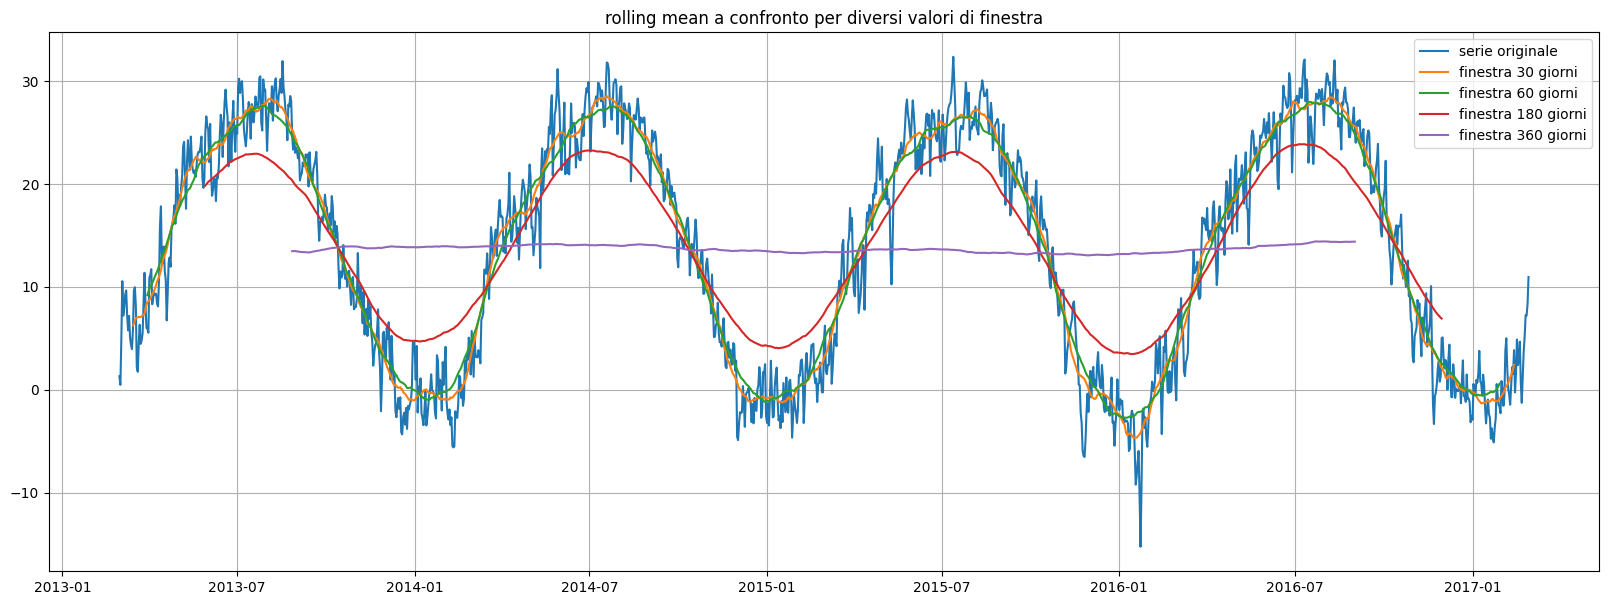
\includegraphics[width=\linewidth,keepaspectratio]{rolling_mean_conf.png}
        \caption{Funzione di rolling mean applicata a diversi valori per la finestra.}
        \label{fig:rolling_mean_conf}
    \end{figure}

\end{esempio}




\subsubsection{Exponential}
Lo smoothing esponenziale è una tecnica di regola empirica 
per ``levigare'' i dati delle serie temporali utilizzando la funzione finestra esponenziale.
Mentre nella rolling mean semplice le osservazioni passate vengono ponderate 
in modo uguale, le funzioni esponenziali vengono utilizzate per assegnare 
pesi esponenzialmente decrescenti nel tempo. 
Si tratta di una procedura di facile apprendimento e di facile applicazione 
per effettuare alcune determinazioni basate su ipotesi precedenti dell'utente, 
come la stagionalità~\cite{wiki:exp_smot}.


\subsubsection{Double Exponential}